\documentclass[twocolumn,twoside,11pt,a4paper]{article}


\usepackage[portuguese]{babel}  % if you want portuguese
\usepackage{graphicx}           % images: .png or .pdf w/ pdflatex; .eps w/ latex

\usepackage{lipsum}             % generate dummy text throughout this template

%% For iso-8859-1 (latin1), comment next line and uncomment the second line
\usepackage[utf8]{inputenc}
%\usepackage[latin1]{inputenc}

\usepackage[T1]{fontenc}        % T1 fonts
\usepackage{lmodern}            % fonts
\usepackage[sc]{mathpazo}       % Use the Palatino font
\linespread{1.05}               % Line spacing - Palatino needs more space between lines
\usepackage{microtype}          % Slightly tweak font spacing for aesthetics
\usepackage{url}                % urls
\usepackage[hang, small, labelfont=bf,up,textfont=it,up]{caption} % Custom captions under/above floats in tables or figures
\usepackage{booktabs}           % Horizontal rules in tables
\usepackage{float}              % Required for tables and figures in the multi-column environment - they need to be placed in specific locations with the [H] (e.g. \begin{table}[H])
\usepackage{paralist}           % Used for the compactitem environment which makes bullet points with less space between them

% geometry package
\usepackage[outer=20mm,inner=20mm,vmargin=15mm,includehead,includefoot,headheight=15pt]{geometry}
%% space between columns
\columnsep 10mm

\usepackage{abstract}           % Allows abstract customization
\renewcommand{\abstractnamefont}{\normalfont\bfseries} % Set the "Abstract" text to bold
\renewcommand{\abstracttextfont}{\normalfont\small\itshape} % Set the abstract itself to small italic text

% \usepackage{titlesec}           % Allows customization of titles
% \renewcommand\thesection{\Roman{section}} % Roman numerals for the sections
% \renewcommand\thesubsection{\Roman{subsection}} % Roman numerals for subsections
% \titleformat{\section}[block]{\large\scshape\centering}{\thesection.}{1em}{} % Change the look of the section titles
% \titleformat{\subsection}[block]{\large}{\thesubsection.}{1em}{} % Change the look of the section titles

\usepackage[pdftex]{hyperref}
\hypersetup{%
    %a4paper = true,              % use A4 paper 
    bookmarks = true,            % make bookmarks 
    colorlinks = true,           % false: boxed links; true: colored links
    pdffitwindow = false,        % page fit to window when opened
    pdfpagemode = UseNone,       % do not show bookmarks
    pdfpagelayout = SinglePage,  % displays a single page
    pdfpagetransition = Replace, % page transition
    linkcolor=blue,              % hyperlink colors
    urlcolor=blue,
    citecolor=blue,
    anchorcolor=green
}

\usepackage{listings} 			%usado para inclusão do xml
\usepackage{textcomp}
\usepackage{indentfirst}         % indent also 1st paragraph


\usepackage{titlesec}

\titlespacing\section{0pt}{12pt plus 4pt minus 2pt}{0pt plus 2pt minus 2pt}


\usepackage{fancyhdr}            % Headers and footers
\pagestyle{fancy}                % pages have headers and footers
\fancyhead{}                     % Blank out the default header
\fancyfoot{}                     % Blank out the default footer
\fancyhead[LO,RE]{Smart-Nutrition} % Custom header text
\fancyhead[RO,LE]{\thepage}      % Custom header text
\fancyfoot[RO,LE]{LAPD — Grupo 01, \today} % Custom footer text 
\renewcommand{\headrulewidth}{0.4pt}
\renewcommand{\footrulewidth}{0.4pt}

%\hyphenation{}                  % explicit hyphenation

\usepackage{color}
\definecolor{gray}{rgb}{0.4,0.4,0.4}
\definecolor{darkblue}{rgb}{0.0,0.0,0.6}
\definecolor{cyan}{rgb}{0.0,0.6,0.6}

\lstset{
  basicstyle=\ttfamily,
  columns=fullflexible,
  showstringspaces=false,
  commentstyle=\color{gray}\upshape
}

\lstdefinelanguage{XML}
{
  morestring=[b]",
  morestring=[s]{>}{<},
  morecomment=[s]{<?}{?>},
  stringstyle=\color{black},
  identifierstyle=\color{darkblue},
  keywordstyle=\color{cyan},
  morekeywords={xmlns,version,type,dateStart,unit,dateEnd,date,hour,id,name}% list your attributes here
}

%----------------------------------------------------------------------------------------
%	macro definitions
%----------------------------------------------------------------------------------------

% entities
\newcommand{\class}[1]{{\normalfont\slshape #1\/}} 
\newcommand{\svg}{\class{SVG}}
\newcommand{\scada}{\class{SCADA}}
\newcommand{\scadadms}{\class{SCADA/DMS}}

%----------------------------------------------------------------------------------------
%	TITLE SECTION
%----------------------------------------------------------------------------------------

\title{\vspace{-15mm}\fontsize{24pt}{10pt}\selectfont\textbf{Smart-Nutrition}} % Article title

\author{Jorge Reis\\
\small \texttt{ei08053@fe.up.pt}\\
\and
Nelson Pereira\\
\small \texttt{ei09025@fe.up.pt}
\and
Tiago Coelho\\
\small \texttt{ei11012@fe.up.pt}\\
\and
Rui Carvalho\\
\small \texttt{ei11024@fe.up.pt}\\
\vspace{-5mm}
}

\date{\today}

%----------------------------------------------------------------------------------------
\usepackage{verbatim}
\begin{document}
\maketitle
\thispagestyle{plain}            % no headers in the first page

%----------------------------------------------------------------------------------------
%	ABSTRACT
%----------------------------------------------------------------------------------------

\begin{abstract}
A aplicação \textit{Smart-Nutrition} surge num contexto de ferramenta de controlo de alimentação como possível complemento ao exercício físico, bem como auxiliar para indivíduos com variados problemas de saúde relacionados direta ou indiretamente com a alimentação. Esta aplicação permite a um utilizador controlar a sua alimentação e evolução corporal, mantendo um histórico dos seus dados antropométricos, consulta de dados nutricionais sobre alimentos, bem como planos alimentares à medida dos seus objetivos pessoais. A aplicação foi desenvolvida com recurso à plataforma eXist-db, mantendo os dados em formato XML numa base de dados nativa. A fonte de dados nutricionais utilizada pela aplicação provém do Departamento de Agricultura Norte Americano.
\end{abstract}

%----------------------------------------------------------------------------------------
%	ARTICLE CONTENTS
%----------------------------------------------------------------------------------------

\section{Introdução}\label{sec:intro}

A sedentarização da população mundial tem-se tornado num fator caracterizador e preocupante, sendo a falta de tempo necessária para manter uma alimentação saudável e a reduzida prática de exercício físico um dos principais obstáculos.
Vários problemas de saúde podem advir deste conjunto de condições, pelo que a adoção de bons hábitos alimentares é um passo importante para a redução desses riscos.
A aplicação \textit{Smart-Nutrition} surge deste modo com o objetivo do controlo calculado e inteligente das refeições efetuadas, permitindo estabelecer novos hábitos alimentares baseados na escolha de alimentos saudáveis e de uma eficiente planificação diária de refeições.

Após a definição do modelo do domínio com base na fonte de dados utilizada, e definição dos objetivos da aplicação, foi realizada uma análise ao estado da arte. As restantes secções do documento apresentam toda a informação sobre os requisitos funcionais da aplicação, a arquitetura da solução implementada, bem como alguns detalhes pertinentes de implementação. A secção final detalha a avaliação das tecnologias usadas, bem como da própria aplicação.


%------------------------------------------------

\section{Fonte de Dados}
A fonte de dados utilizada é uma base de dados nutricional pertencente ao \textit{United States Department of Agriculture — Agricultural Research Service} (USDA) \cite{usda}, o que lhe confere boa reputação. A NDB (\textit{National Nutrient Database for Standard Reference}) \cite{ndb} possui uma enorme quantidade de alimentos, segmentados por grupos alimentares, contendo os valores nutricionais e calóricos para diferentes unidades de medida. Os principais dados estão disponíveis para \textit{download} em formatos de ficheiro ASCII ou CSV, mas com limitações. No entanto, através de uma API REST disponibilizada pelo USDA é possível aceder a toda a base de dados permitindo vários tipos de pedidos personalizados de informação nutricional para um dado alimento, incluindo escolha dos nutrientes pretendidos, diferentes unidades de medida (uma chávena, uma colher, o \textit{standard} 100g, por exemplo), aliados a diferentes estados dos alimentos (ralado, derretido, por exemplo) e ordenação por valores de um nutriente.
Os pedidos à API da USDA podem ser retornados em formato JSON ou XML, sendo que é utilizado XML por ser o tipo de linguagem utilizado nos restantes dados armazenados localmente.


\section{Modelo de Domínio}
Concetualmente, existem 2 categorias principais de dados a serem tratadas e acedidas. Como suporte às principais funcionalidades da aplicação é armazenada toda a informação nutricional relacionada com cada alimento para várias unidades de medida, assim como partição dos alimentos por grupo alimentar. Por outro lado, existe a informação relacionada com os utilizadores da aplicação. Serão armazenados, para além de alguns dados pessoais, registos de medições realizadas regularmente (peso, altura, índice de massa corporal, entre outros) e sobretudo os planos alimentares criados pelo utilizador para cada dia.


\section{Objetivos}
A aplicação web desenvolvida propõe-se, enquanto objetivo principal, a apoiar o planeamento das refeições do utilizador de modo a que as mesmas se adequem às suas necessidades, segundo um conjunto de nutrientes e restrições calóricas estipuladas.  Assim, os utilizadores registados na aplicação terão a possibilidade de manter, para além de alguns dados pessoais, um histórico dos seus valores antropométricos e respetiva evolução, realizar pesquisas por alimentos e observar os seus valores nutricionais para várias unidades de medida, assim como realizar planos alimentares mantendo um controlo aproximado dos nutrientes e calorias a ingerir diariamente e por refeição.


\section{Estado da arte}
Com o objetivo de perceber o mercado existente, várias aplicações foram testadas \cite{apps}. Grande parte das mais conhecidas permite a inserção dos valores antropométricos do utilizador, bem como do nível de atividade física por si praticado diariamente, procedendo à sugestão de refeições baseadas nessas caraterísticas. No entanto, poucas são as aplicações testadas que aliam a componente de pesquisa eficaz e independente dos objetivos do utilizador, à componente de diário nutricional e diretamente relacionado com os seus objetivos (por exemplo, perda de gordura, aumento de massa muscular). A maioria destas aplicações também não é particularmente eficaz na pesquisa de alimentos onde exista a filtragem por grupos de alimentos, tipos de nutrientes e quantidade de calorias. Considera-se a motivação um fator importante e, desta forma, a representação gráfica da evolução do utilizador será também importante na aplicação projetada. 
Listam-se, de seguida, as principais funcionalidades avaliadas e quais as principais aplicações estudadas (MyFitnessPal \cite{myfitnesspal}, Nutridata \cite{nutridata}, TecnoNutri \cite{tecnonutri}, MyDietDiary \cite{mydietdiary}, Fooducate \cite{fooducate}) que as implementam convenientemente.

\begin{itemize}
 \item   \textbf{Introdução de caraterísticas individuais (valores antropométricos e nível de atividade)} — Regista os referidos dados do utilizador permitindo fazer uma posterior análise comparativa da sua evolução. Neste ponto destacam-se as aplicações MyFitnessPal e TecnoNutri;
 \item    \textbf{Criação de perfis baseados em metas e objetivos} — Avalia o objetivo do utilizador (por exemplo, perda de massa gorda, aumento de massa muscular). Estando relacionado com o anterior, também neste ponto se referem as aplicações MyFitnessPal e TecnoNutri;
 \item   \textbf{Diário alimentar} — Permite efetuar o registo das refeições diárias, sendo contabilizado o consumo calórico/nutricional diário. MyDietDiary e MyFitnessPal mostraram capacidade para o realizar;
 \item    \textbf{Comparação nutricional} — Permite comparar a composição nutricional de diferentes alimentos. Destaca-se a aplicação NutriData (versão paga);
 \item   \textbf{Pesquisa baseada em grupos de alimentos (por exemplo, vegetais, laticínios)} — Mais uma vez se refere a aplicação NutriData (versão paga), que mostra estar  direcionada para pesquisas;
 \item    \textbf{Utilização das porções padrão} — A maioria das aplicações ajustou os resultados da pesquisa ao tipo de alimento;
 \item    \textbf{Lista de favoritos} — Permite um acesso rápido aos alimentos/refeições mais frequentes na dieta do utilizador. Destacam-se as aplicações MyFitnessPal e TecnoNutri;
 \item	  \textbf{Lista de alergéneos} — As aplicações MyFitnessPal, NutriData e Fooducate descrevem os principais alergéneos.
\end{itemize}


\section{Arquitectura da Solução}
A aplicação foi desenvolvida através da plataforma \textit{eXist} \cite{existdb}, que permite a utilização da sua base de dados \textit{XML}, assim como o desenvolvimento integrado da aplicação web.
Assim, em termos de \textit{XML Storage} decidiu-se pela utilização da sua base de dados XML nativa, pois dado o baixo nível de relações entre identidades, considerou-se positiva a utilização de uma solução \textit{NoSQL}. No entanto, na utilização realizada até ao momento, não foram detetados problemas de performance.
A base de dados é populada com ficheiros \textit{XML} segundo os \textit{schemas} apresentados em anexo, sendo que o XML relativo aos alimentos é gerado a partir de um \textit{script Java} que realiza o download em \textit{chunks} dos alimentos presentes na base de dados nutricional da \textit{USDA}, aplicando posteriormente uma transformação através da tecnologia \textit{XSLT} para o formato presente no nosso \textit{schema}. Para utilização da aplicação serão feitas interrogações à base de dados através da linguagem \textit{XQuery}.
Para realização das interfaces da aplicação recorreu-se, para além das tecnologias mais comuns como HTML e CSS, às bibliotecas jQuery e \textit{Bootstrap}, permitindo sobretudo um \textit{responsive layout}, que permite a sua utilização em vários tipos de dispositivos. Assim, o \textit{frontend} da aplicação comunica diretamente com a base de dados através da plataforma \textit{eXist}.


\begin{figure}[h!]
  \centering
      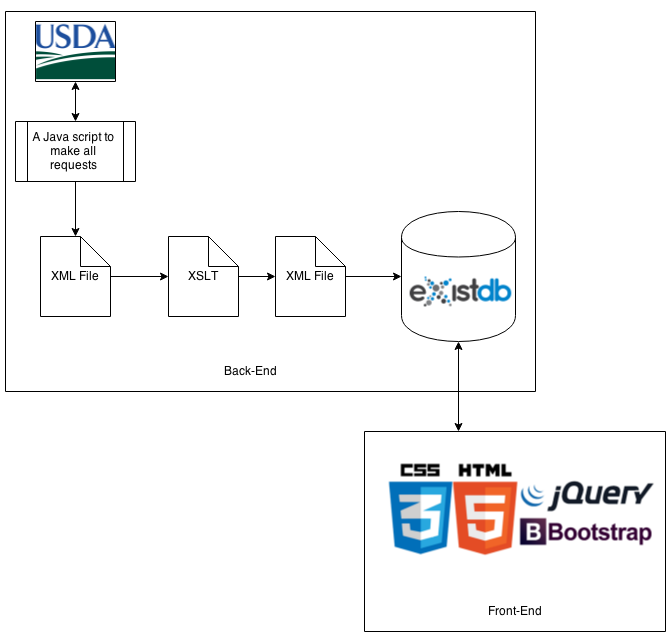
\includegraphics[width=0.5\textwidth]{arquitectura}
  \caption{Descrição da arquitetura da aplicação.}
\end{figure}


\section{Schema da linguagem \textit{XML}}
Perante as informações descritas nas secções anteriores relativamente à base de dados XML, dois ficheiros \textit{XSD} foram definidos. O primeiro representa a estrutura do documento onde é guardada toda a informação do utilizador, os seus dados antropométricos bem como a descrição do planeamento das suas refeições. No segundo ficheiro \textit{XSD} é apresentada a estrutura de toda a informação relativa aos alimentos.
Estes \textit{schemas XML} podem ser observados gráficamente nas figuras \ref{fig:foods_schema} e \ref{fig:user_schema}, em anexo.
Sendo que o ficheiro XML relativo à informação dos alimentos obtido diretamente pela \textit{USDA API} não se encontra no formato definido para a nossa aplicação, este é sujeito a uma transformação XSLT.


\section{Requisitos do utilizador}
A aplicação foi projetada para apenas um tipo de utilizador, tendo este uma conta associada para ser possível o registo dos seus dados e evolução. Relativamente aos requisitos funcionais, apresentam-se os seguintes:

\begin{center}
   \begin{tabular}{ | l | p{1.4cm} | p{3.0cm} | p{1.6cm}  |}
   \hline
   ID & Nome & Descrição & Prioridade \\ \hline
   US101 & Login &  Como Utilizador, quero poder efetuar login para aceder à aplicação. &  Core  \\ \hline
   US102 & Logout &  Como Utilizador Autenticado, quero poder efetuar logout. &  Média  \\ \hline
   US103 & Registo &  Como Utilizador, quero poder registar-me na aplicação &  Core  \\ \hline
   US104 & Pesquisa &  Como Utilizador Autenticado, quero poder pesquisar a informação nutricional de um determinado alimento. &  Core  \\ \hline

      \end{tabular}
\end{center}

\begin{center}
   \begin{tabular}{ | l | p{1.4cm} | p{3.0cm} | p{1.4cm}  |}
   \hline
      US105 & Registar dados &  Como Utilizador Autenticado, quero poder registar a evolução dos meus dados antropométricos. &  Alta  \\ \hline
   US106 & Planos &  Como Utilizador Autenticado, quero poder efetuar planos alimentares. &  Alta  \\ \hline
   US107 & Visualizar Planos &  Como Utilizador Autenticado, quero poder aceder aos meus planos alimentares. &  Alta  \\ \hline
   US108 & Evolução &  Como Utilizador Autenticado, quero visualizar a minha evolução de forma apelativa. &  Alta  \\ \hline
   \end{tabular}
\end{center}


Enquanto requisitos não funcionais, referem-se:

\begin{center}
   \begin{tabular}{ | l | p{2.1cm} | p{4.0cm} | p{1.8cm}  |}
   \hline
   ID & Nome & Descrição \\ \hline
   RNF101 & Aplicação responsiva & A aplicação deve ser acessível e adaptável a diversos dispositivo.  \\ \hline
   RNF102 & Resposta rápida & A aplicação responder rapidamente às pesquisas, reduzindo o mais possível o tempo de espera do utilizador.  \\ \hline
   RNF103 & Sistema multi-plataforma &  O sistema deverá ser executável em qualquer plataforma/\textit{browser}. \\ \hline
   RNF104 & Comunicação com o \textit{eXist} & A aplicação deverá funcionar com comunicação com o \textit{eXist}.\\ \hline
   \end{tabular}
\end{center}


\section{Interrogações e \textit{Updates} à base de dados XML}
Como base da aplicação temos as interrogações e \textit{updates} ao domínio, presente na base de dados \textit{eXist}. A maior parte assenta em informações relacionadas com alimentos e com o utilizador da aplicação. Assim, realçam-se as seguintes:

\begin{itemize}
	\item Quais os alimentos que têm um determinado elemento textual no seu nome?
  \item Qual é a informação nutricional de um determinado alimento?
  \item Quais são unidades de medida associadas a um determinado alimento?
  \item Quais são os dados antropométricos actuais e anteriores do utilizador?
    \item Qual o \textit{intake} calórico diário aconselhado para o utilizador, em função dos seus dados antropométricos e nível de atividade física?
  \item Quais são os planos alimentares do utilizador?
  \item Inserção de novos registos antropométricos.
  \item Inserção de novos planos alimentares.
\end{itemize}


\section{Detalhes de implementação}
Relativamente às \textit{queries} de pesquisa de informação, estas foram realizadas usando código \textit{XQuery}, \textit{updates} e \textit{deletes} foram implementados usando a extensão de \textit{update} \cite{update_ext} da \textit{eXist-db}. A troca de informação entre \textit{front-end} e \textit{back-end} ocorre pela invocação de funções \textit{xquery}. Estas funções retornam os resultados diretamente para o código \textit{html}.




\section{Avaliação do trabalho e das tecnologias}\label{sec:conclusions}

Como ambiente de desenvolvimento web, a plataforma \textit{exist} revela-se pouco prática e flexivel em termos de comunicação entre o \textit{front-end} e \textit{back-end}. Relativamente ao tipo de base de dados \textit{xml} utilizada, apesar de parecer uma opção válida, uma melhor solução teria sido uma base de dados relacional, devido à granularidade dos dados armazenados.

Em termos de trabalho futuro e pela investigação sobre o estado da arte, verifica-se que perante o mercado de aplicações de nutrição há falta de uma componente autónoma que indique alimentos baseados nos objetivos do utilizador. A resolução deste problema passava por uma investigação algorítmica, bem como por uma procura mais extensa relativamente a informações nutricionais que assentem nas necessidades nutritivas e calóricas em concordância com os objetivos dos diferentes utilizadores (aumento de massa muscular, redução da percentagem de gordura corporal ou redução de peso indiscriminado).


%----------------------------------------------------------------------------------------
%	REFERENCE LIST
%----------------------------------------------------------------------------------------

%% auto bibliographic list 
\renewcommand{\bibname}{Referências}
\begin{thebibliography}{9}


\bibitem{usda}
  \emph{United States Department of Agriculture}.
  http://www.usda.gov/,
  online em 29 Abril 2015.

\bibitem{ndb}
  USDA — Agricultural Research Service,
  \emph{National Nutrient Database for Standard Reference}.
  http://ndb.nal.usda.gov/ndb/doc/index,
  online em 29 Abril 2015.
  
  \bibitem{apps}
  John Corpuz,
  \emph{Nutrition Apps}.
  http://www.tomsguide.com/us/best-diet-nutrition-apps,review-2308.html,
  13 Janeiro 2015.
  
  \bibitem{myfitnesspal}
  \emph{MyFitnessPal}.
  https://www.myfitnesspal.com/,
  online em 25 Março 2015.
  
   \bibitem{nutridata}
  \emph{NutriData}.
  http://nutridata.mgoyanes.com/,
  online em 25 Março 2015.
  
   \bibitem{tecnonutri}
  \emph{TecnoNutri}.
  http://www.tecnonutri.com.br/,
  online em 25 Março 2015.
  
  \bibitem{mydietdiary}
  \emph{MyDietDiary}.
  http://www.medhelp.org/land/calorie-counter-app,
  online em 25 Março 2015.
  
  \bibitem{fooducate}
  \emph{Fooducate}.
  http://www.fooducate.com/,
  online em 25 Março 2015.
  
  \bibitem{existbook}
  Erik Siegel, Adam Retter,
  \emph{eXist — A NoSQL Document Database and Application Platform}.
  O'Reilly Media,
  2014.
  
    \bibitem{existdb}
     eXist Solutions,
  \emph{eXistdb — The Open Source Native XML Database}.
  http://exist-db.org/,
  online em 29 Abril 2015.


\bibitem{update_ext}
     eXist Solutions,
  \emph{XQuery Update Extension}.
  http://exist-db.org/exist/apps/doc/update\_ext.xml,
  online em 03 de Junho 2015.
  
 
  
  
\end{thebibliography}

%----------------------------------------------------------------------------------------
\newpage
\clearpage
\appendix
\chapter{\huge{Anexos}}

\clearpage

\section{Diagramas de Schema}
\clearpage

\begin{figure}
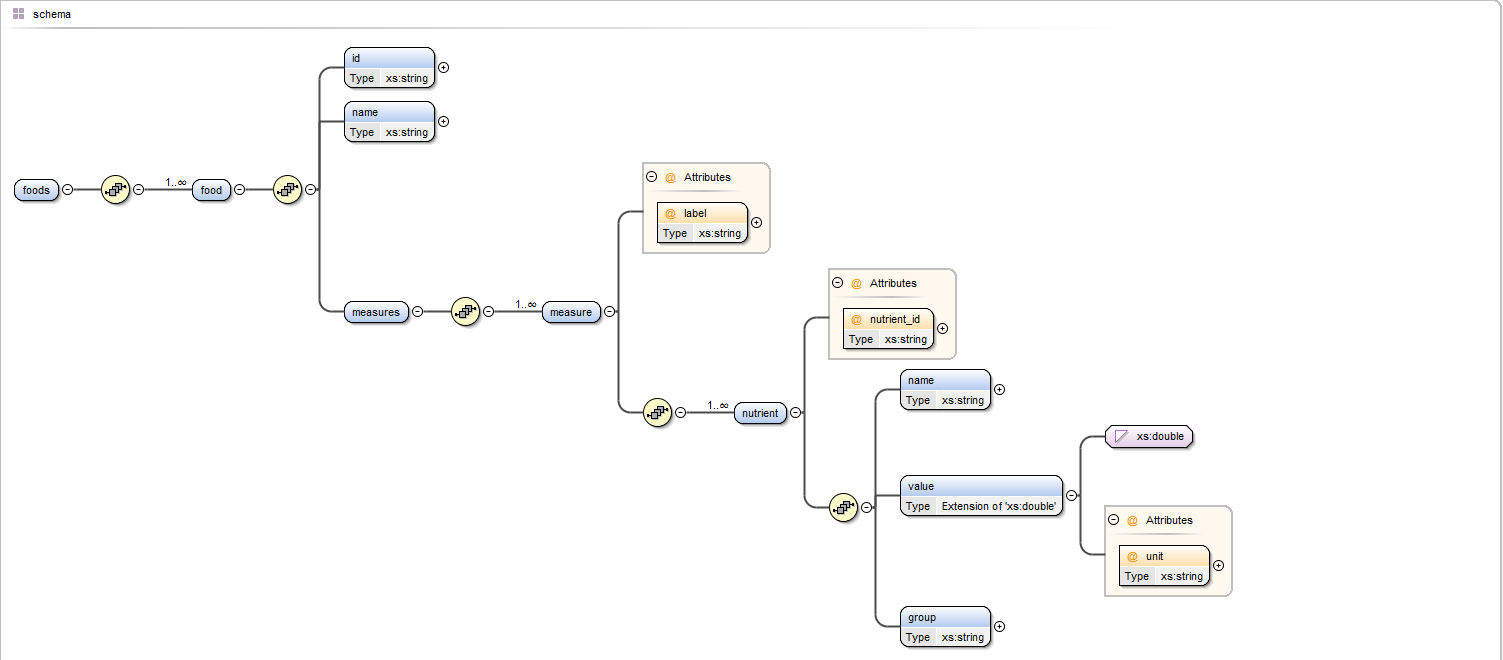
\includegraphics[scale=0.56]{foods_schema}
    \caption{Ficheiro schema referente aos alimentos}
    \label{fig:foods_schema}
\end{figure}

\clearpage

\begin{figure}
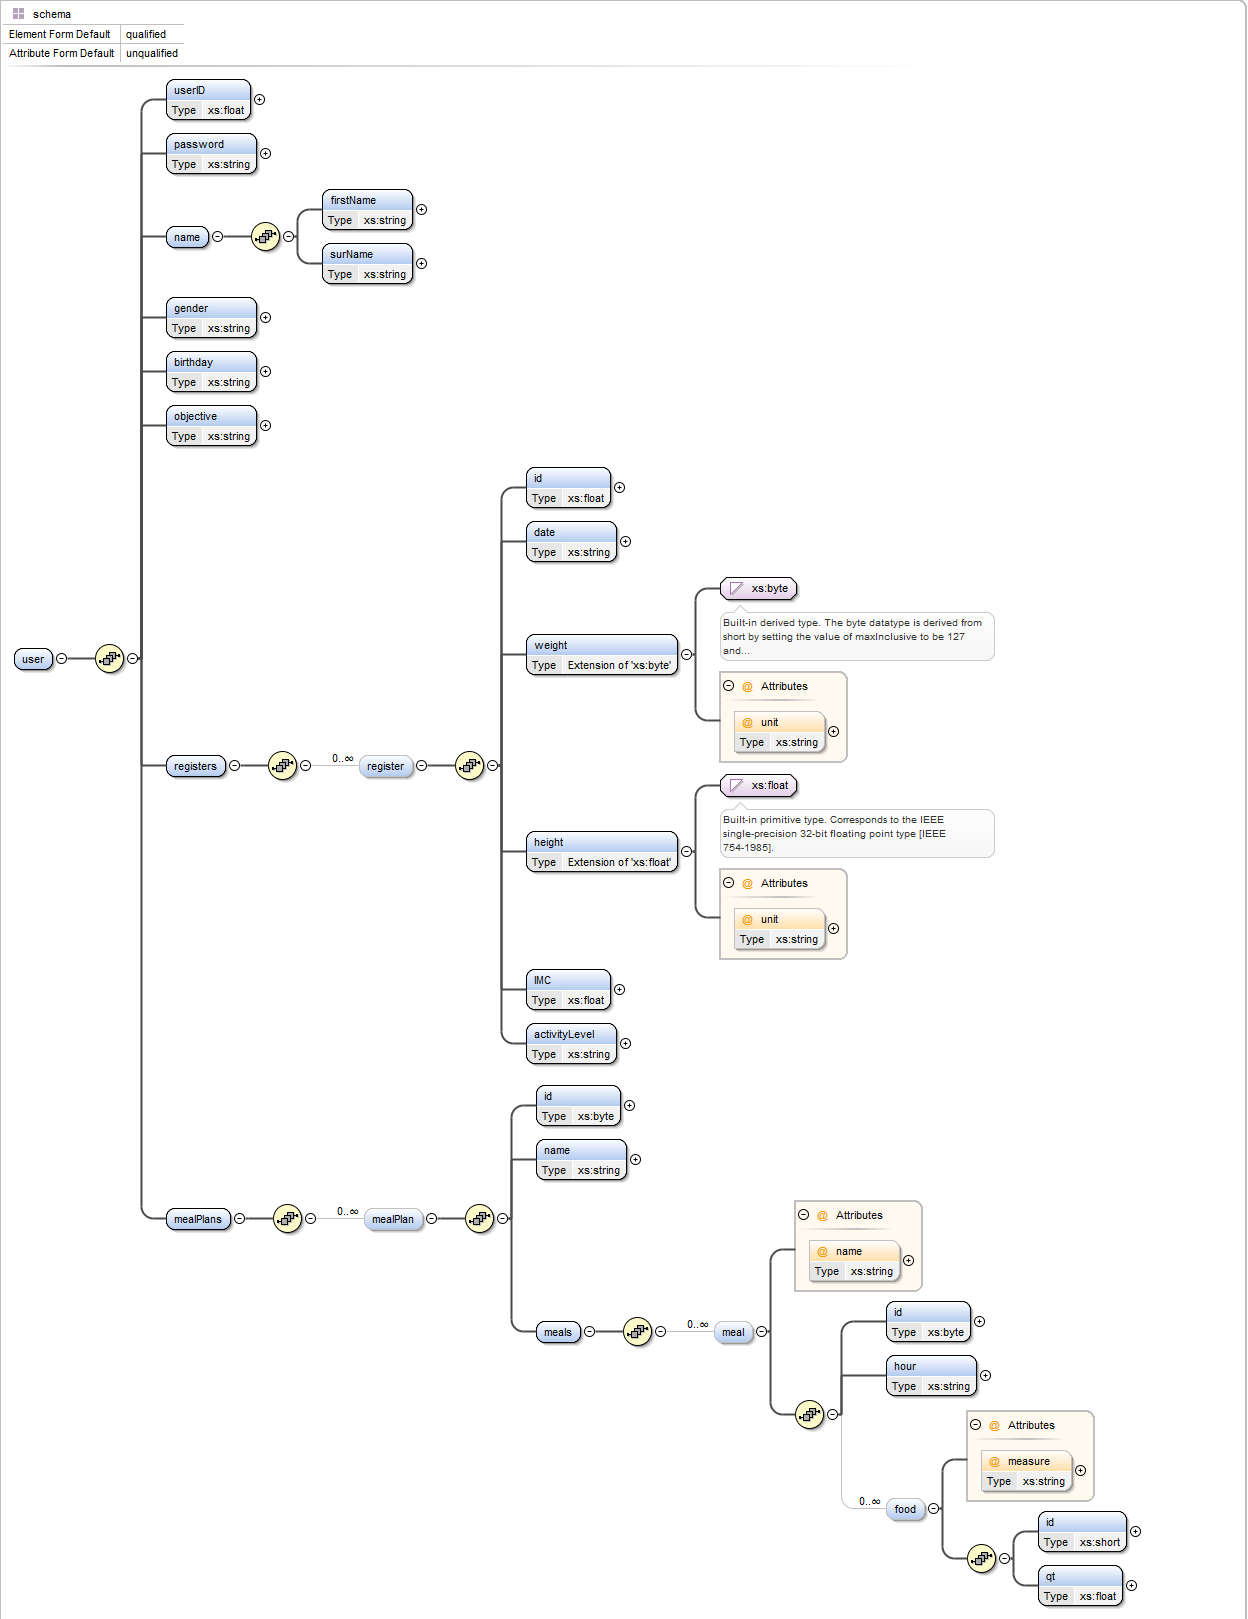
\includegraphics[scale=0.42]{user_schema}
\caption{Ficheiro schema referente aos utilizadores}
\label{fig:user_schema}
\end{figure}
\clearpage



\onecolumn
\section{Manual de Utilização}
Após ter efetuado o login, o utilizador será reencaminhado para a página geral da aplicação, correspondente à "Dashboard", que tem uma estrutura de consulta rápida das diferentes funcionalidades da aplicação.
É imediatamente mostrada uma barra de pesquisa de alimentos, para confortável obtenção dos dados nutricionais do alimento pretendido, bem como indicado o estado atual do utilizador no que concerne à sua evolução física de acordo com as variáveis a ela associadas.

Ainda na dashboard, são também listados os seus planos para o dia atual de modo a permitir uma rápida consulta.
Acedendo à secção "Anthropometric Data", são mostrados os dados antropometricos correspondentes à data da última introdução, e permitida uma nova inserção destes dados (altura e peso). 
Na secçao "Search", o utilizador poderá introduzir o nome do alimento para o qual pretende saber detalhes nutricionais, sendo-lhe devolvida uma lista de todos os alimentos que contêm a palavra pesquisada. Bastar-lhe-á encontrar o alimento pretendido e carregar em "More Info" para ter acesso aos detalhes.
Tendo acedido aos detalhes de alimento, poderá ver a informação em forma de tabela na qual as colunas correspondem a Medida, Nutriente, Valor (quatidade por medida), e Grupo de Nutriente. Cada linha corresponderá, naturalmente, a cada um dos nutrientes do alimento.

\onecolumn
\section{Imagens da Aplicação}

\clearpage

\begin{figure}
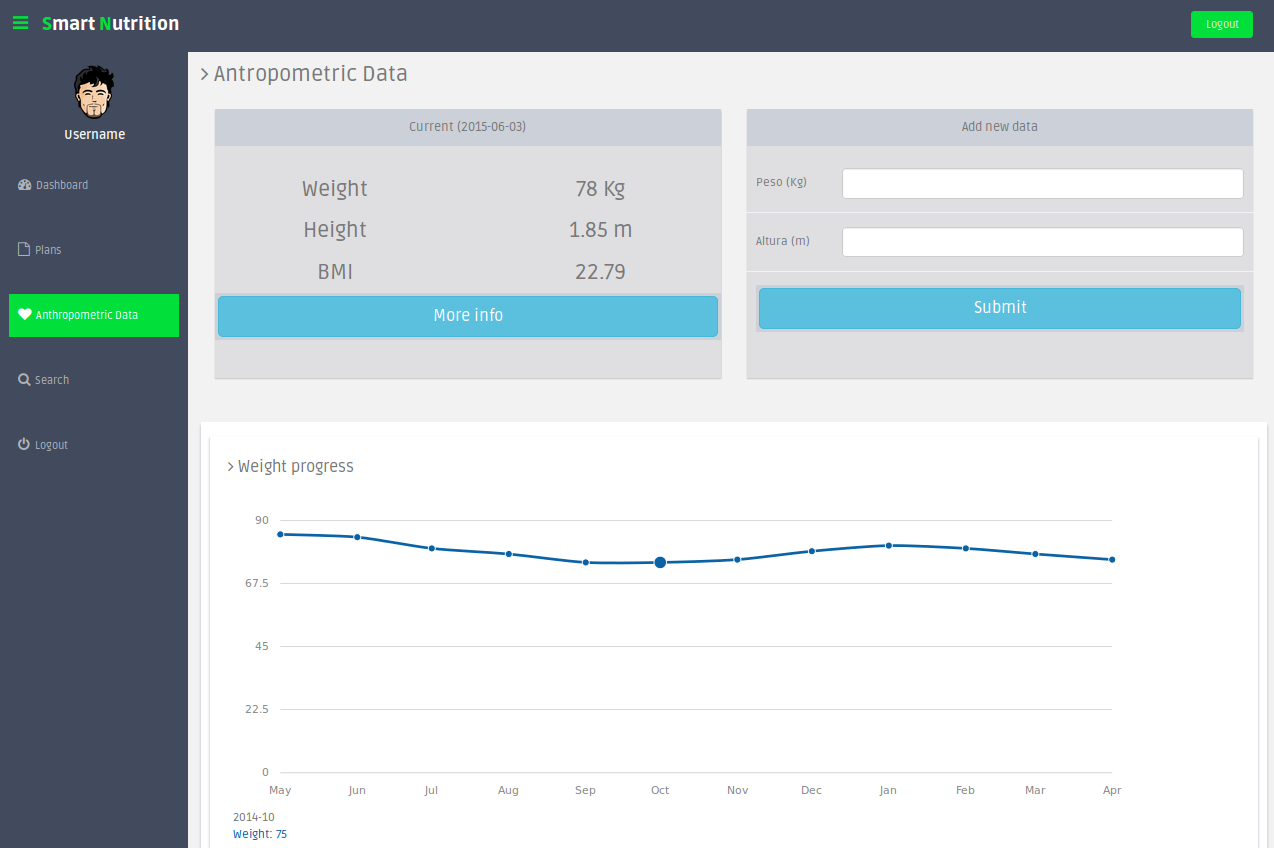
\includegraphics[scale=0.38]{antropometricos}
\caption{Página dos dados antropométricos do utilizador}
\label{fig:antropometricos}
\end{figure}

\begin{figure}
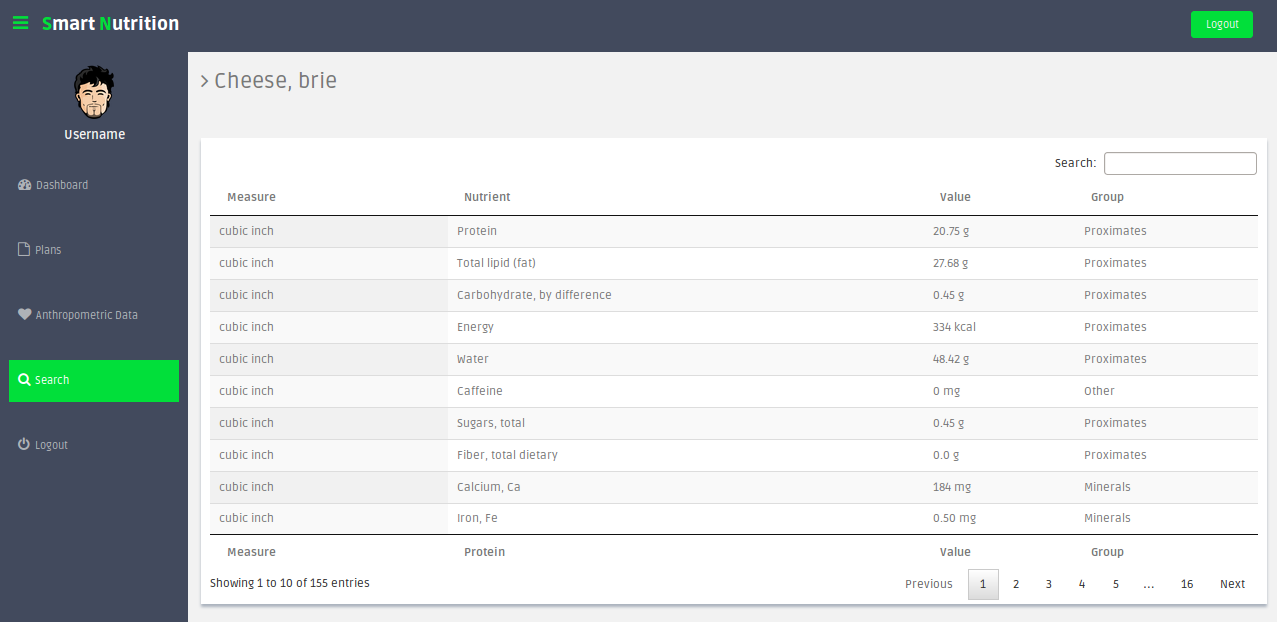
\includegraphics[scale=0.38]{food}
\caption{Informação dos nutrientes e calorias associados a um alimento}
\label{fig:food}
\end{figure}

\begin{figure}
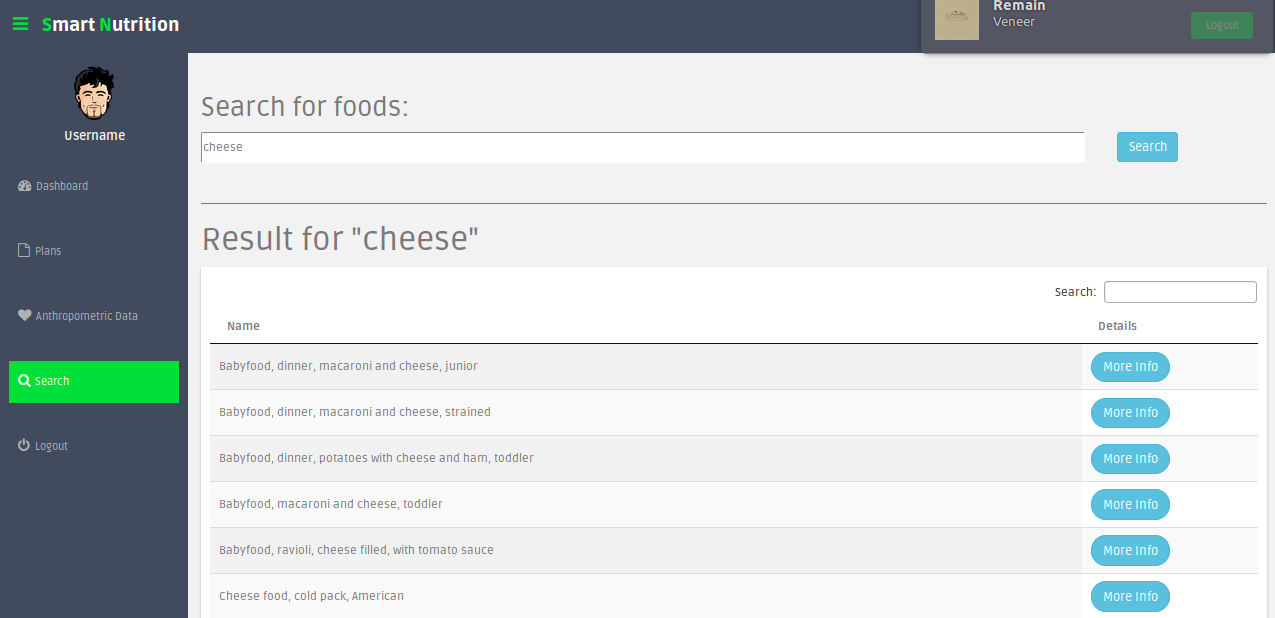
\includegraphics[scale=0.38]{search}
\caption{Página de pesquisa de alimentos}
\label{fig:search}
\end{figure}

\begin{figure}
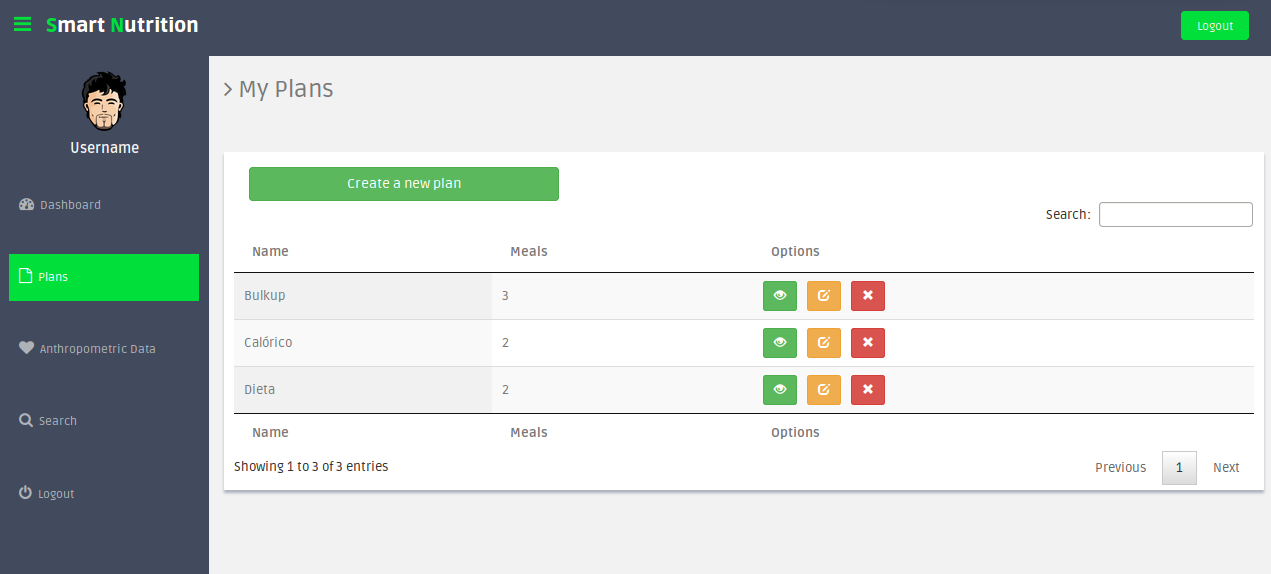
\includegraphics[scale=0.38]{plans}
\caption{Página dos planos de alimentação atuais}
\label{fig:plans}
\end{figure}



\end{document}